\documentclass[9pt,twocolumn]{paper-template}
% Use the lineno option to display guide line numbers if required.

\usepackage{lipsum}
\templatetype{twocolumn} % Choose template 
% {pnasresearcharticle} = Template for a two-column research article
% {pnasmathematics} %= Template for a one-column mathematics article
% {pnasinvited} %= Template for a PNAS invited submission

\title{Libet's Experiment: [Add your custom title here]}

% Use letters for affiliations, numbers to show equal authorship (if applicable) and to indicate the corresponding author
\author[a,b]{Author One}
\author[b,c]{Author Two} 
\author[a]{Author Three}

\affil[a]{Student, Department, Sharif University of Technology}
\affil[b]{Affiliation Two}
\affil[c]{Affiliation Three}

% Please add here a significance statement to explain the relevance of your work
\significancestatement{You are encouraged to submit a 120-word maximum statement about the significance of your paper written at a level understandable to an undergraduate educated scientist outside their field of speciality. The primary goal of the Significance Statement is to explain the relevance of the work in broad context to a broad readership. The Significance Statement appears in the paper itself and is required for all research papers in some journals.}

% Please include corresponding author, author contribution and author declaration information
\authorcontributions{Please provide details of author contributions here.}
\equalauthors{\textsuperscript{1}A.O.(Author One) and A.T. (Author Two) contributed equally to this work (remove if not applicable).}

% Keywords are not mandatory, but authors are strongly encouraged to provide them. If provided, please include two to five keywords, separated by the pipe symbol, e.g:
\keywords{Keyword 1 $|$ Keyword 2 $|$ Keyword 3 $|$ ...} 

\begin{abstract}
Please provide an abstract of no more than 250 words in a single paragraph. Abstracts should explain to the general reader the major contributions of the article. References in the abstract must be cited in full within the abstract itself and cited in the text.
\end{abstract}

\dates{This manuscript was compiled on \today}

\begin{document}

\maketitle
\thispagestyle{firststyle}
\ifthenelse{\boolean{shortarticle}}{\ifthenelse{\boolean{singlecolumn}}{\abscontentformatted}{\abscontent}}{}

% If your first paragraph (i.e. with the \dropcap) contains a list environment (quote, quotation, theorem, definition, enumerate, itemize...), the line after the list may have some extra indentation. If this is the case, add \parshape=0 to the end of the list environment.
\dropcap{T}his template is provided to help you write your work in the correct journal format.  Instructions for use are provided below. The introduction should contain three paragraphs. Paragraph one: give a background
to the problem. Paragraph two: what is already done
what issues remain. Paragraph three how you are
proposing to address it in this paper.
Note: please start your introduction without including the word ``Introduction'' as a section heading; this heading is implied in the first paragraphs. Many find it useful to organize their manuscripts with the following order of sections;  Title, Author Affiliation, Keywords, Abstract, Significance Statement, Results, Discussion, Materials and methods, Acknowledgments, and References. Other orders and headings are permitted. 

\section*{Results}
Go over your analysis/experiments step by step and
describe what is shown in each figure then make a case
to go to the next analysis.\\

(dummy text)\lipsum[1]

\section*{Discussion}
Should be at least three paragraphs: first paragraph says what
was the main results you showed, second paragraph says
what was the relationship of what you showed to what
was previously shown in other papers and what might
be the shortcomings of your approach, third paragraph
gives a short summary of significance of what you found
and future directions.\\

(dummy text)\lipsum[1]

\begin{figure}%[tbhp]
\centering
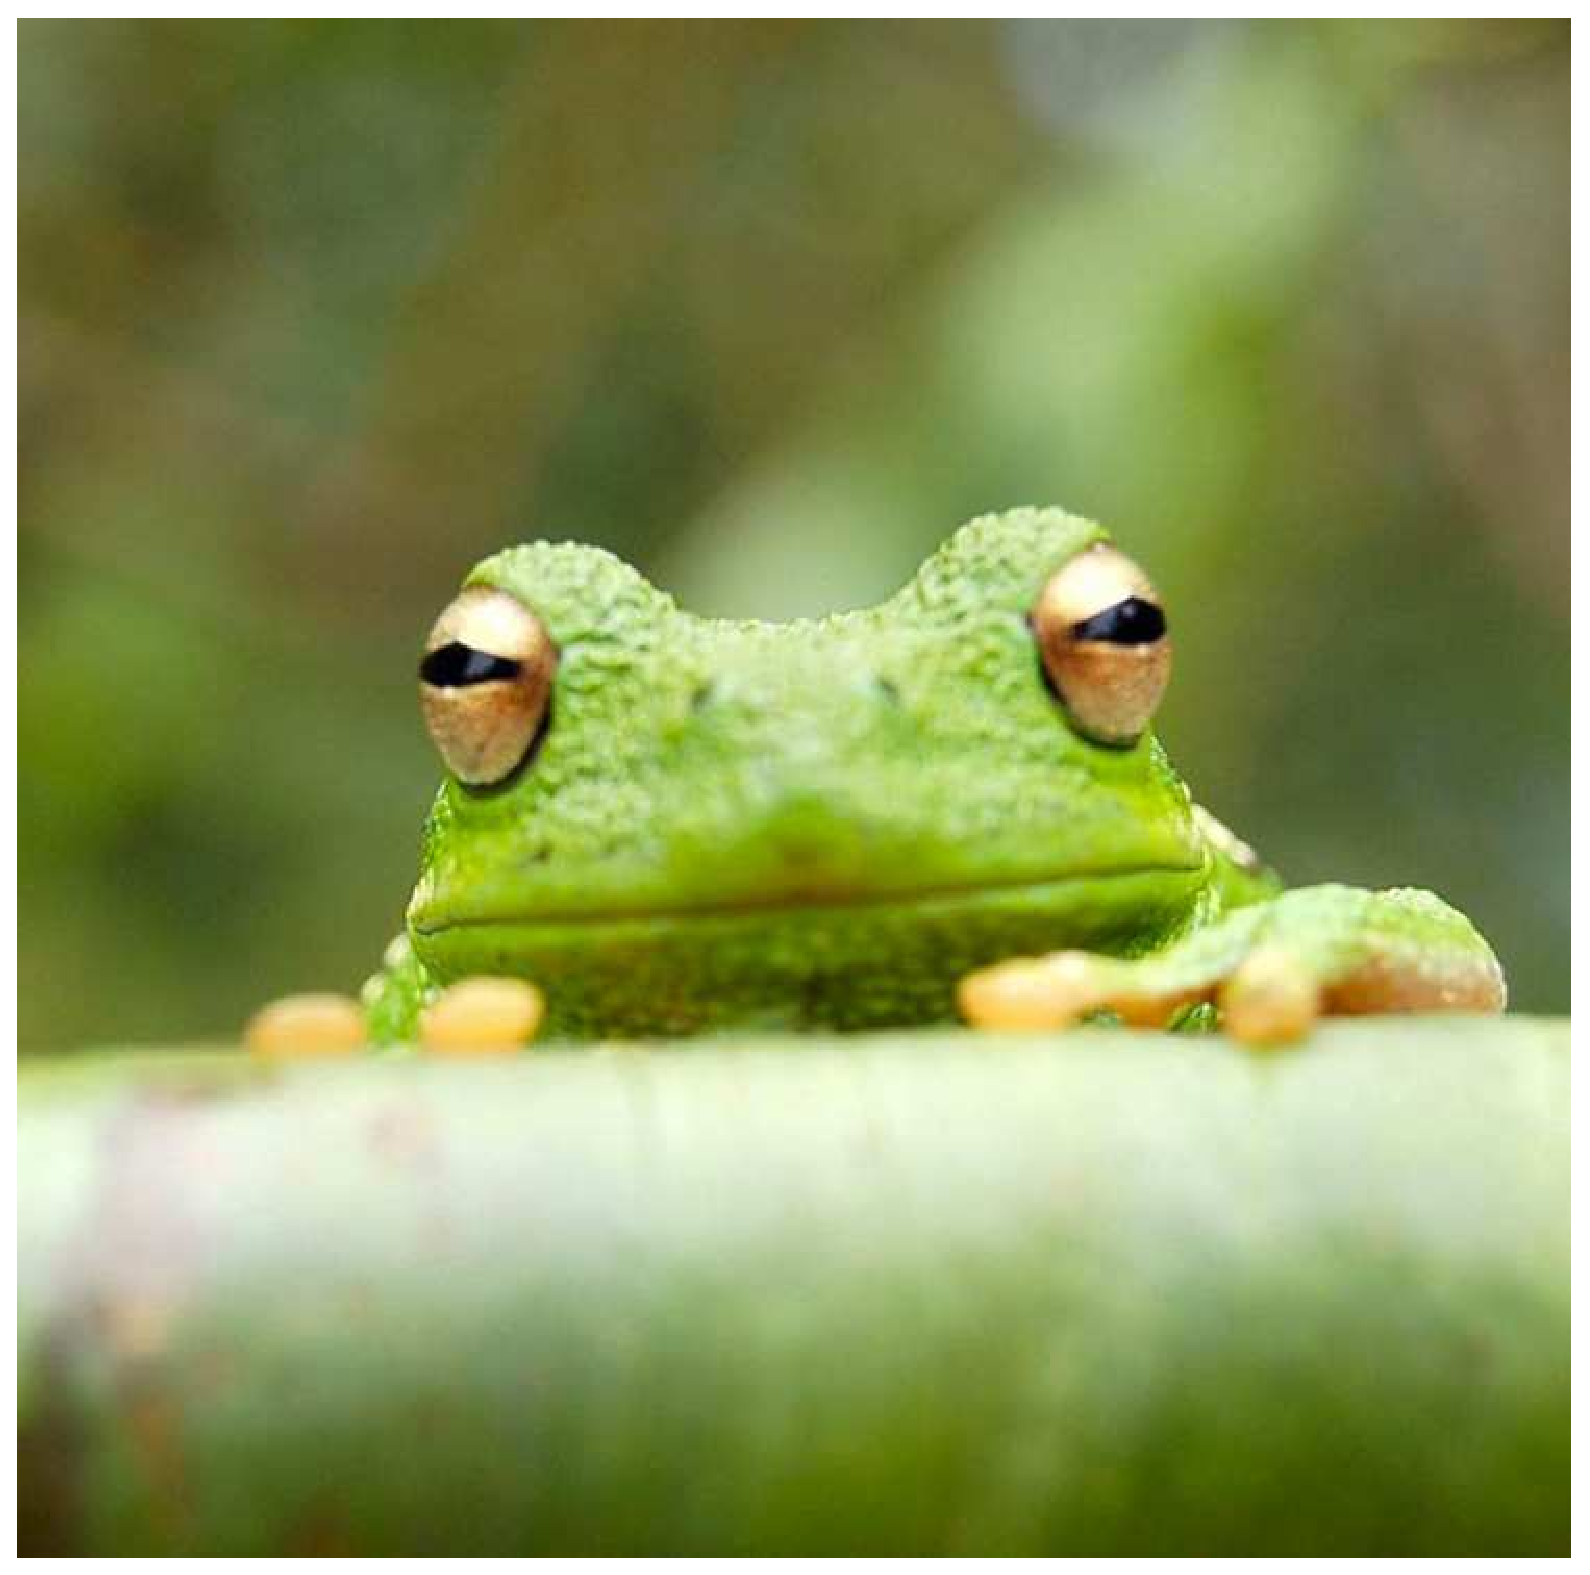
\includegraphics[width=.8\linewidth]{frog}
\caption{Placeholder image of a frog with a long example caption to show justification setting.}
\label{fig:frog}
\end{figure}


\begin{SCfigure*}[\sidecaptionrelwidth][t]
\centering
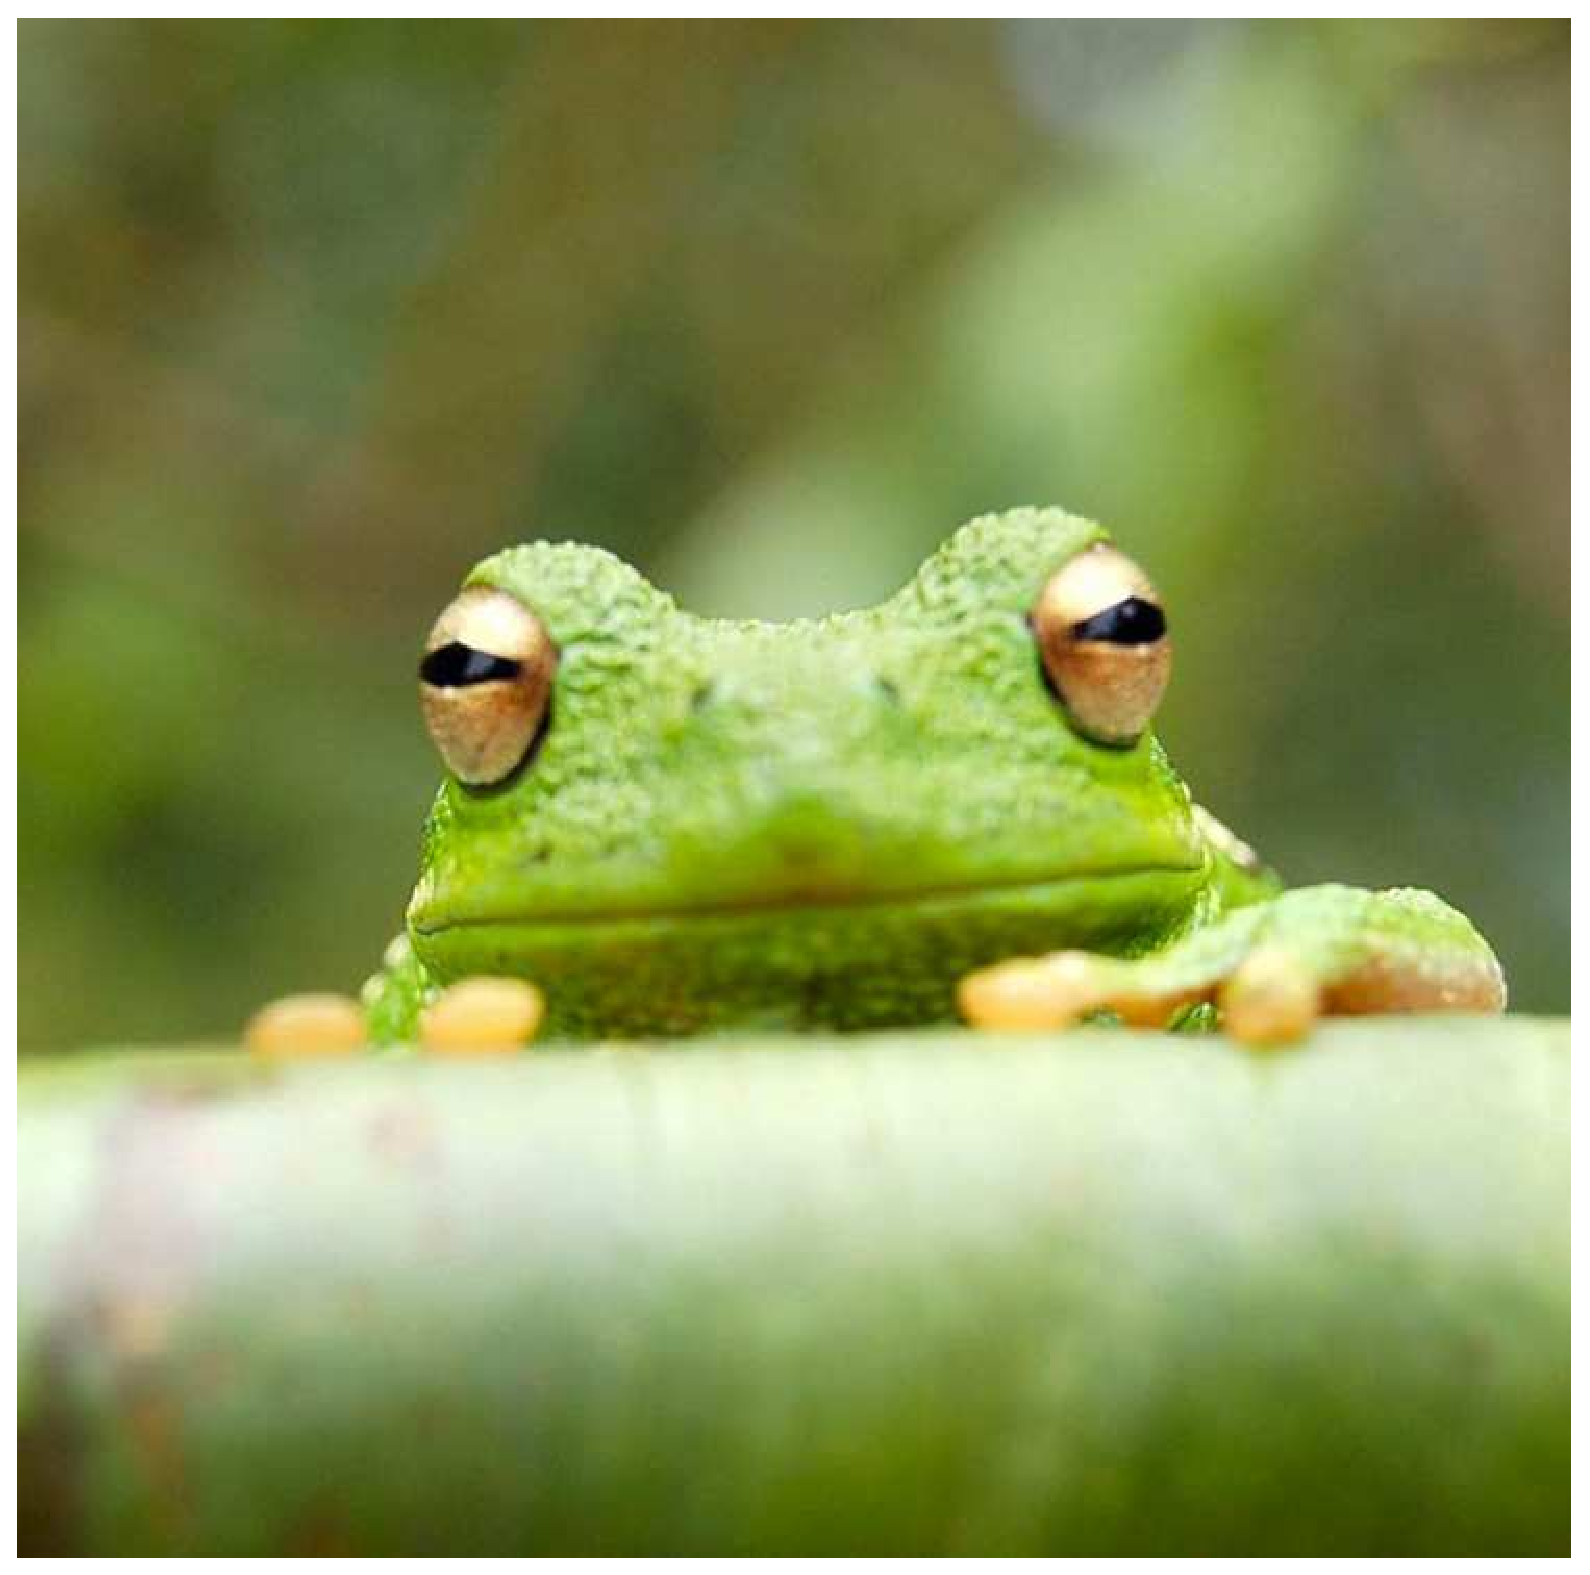
\includegraphics[width=11.4cm,height=11.4cm]{frog}
\caption{This caption would be placed at the side of the figure, rather than below it.}\label{fig:side}
\end{SCfigure*}

\section*{Materials and Methods}
Describe your data acquisition, dataset, analysis in details.

\subsection*{Manuscript Length}
Less than ten pages using a two-column format.

\subsection*{References}
References should be cited in numerical order as they appear in text; this will be done automatically via bibtex, e.g. \cite{belkin2002using} and \cite{berard1994embedding,coifman2005geometric}. 

\subsection*{Single column equations}

You may use 1- or 2-column equations in your article, according to your preference.

To allow an equation to span both columns, use the \verb|\begin{figure*}...\end{figure*}| environment mentioned above for figures.

Note that the use of the \verb|widetext| environment for equations is not recommended, and should not be used. 

\begin{figure*}[bt!]
\begin{align*}
(x+y)^3&=(x+y)(x+y)^2\\
       &=(x+y)(x^2+2xy+y^2) \numberthis \label{eqn:example} \\
       &=x^3+3x^2y+3xy^3+x^3. 
\end{align*}
\end{figure*}
\subsection*{Digital Figures}

Only TIFF, EPS, and high-resolution PDF are allowed for figures that will appear in the main text, and images must be final size. Color images must be in RGB (red, green, blue) mode.
Figures and Tables should be labelled and referenced in the standard way using the \verb|\label{}| and \verb|\ref{}| commands.
Figure \ref{fig:frog} shows an example of how to insert a column-wide figure. To insert a figure wider than one column, please use the \verb|\begin{figure*}...\end{figure*}| environment. Figures wider than one column should be sized to 11.4 cm or 17.8 cm wide. Use \verb|\begin{SCfigure*}...\end{SCfigure*}| for a wide figure with side captions.

\subsection*{Tables}
In addition to including your tables within this manuscript file.

\begin{table}%[tbhp]
\centering
\caption{Comparison of the fitted potential energy surfaces and ab initio benchmark electronic energy calculations}
\begin{tabular}{lrrr}
Species & CBS & CV & G3 \\
\midrule
1. Acetaldehyde & 0.0 & 0.0 & 0.0 \\
2. Vinyl alcohol & 9.1 & 9.6 & 13.5 \\
3. Hydroxyethylidene & 50.8 & 51.2 & 54.0\\
\bottomrule
\end{tabular}

\addtabletext{nomenclature for the TSs refers to the numbered species in the table.}
\end{table}

\acknow{Please include your acknowledgments here, set in a single paragraph. Please do not include any acknowledgments in the Supporting Information, or anywhere else in the manuscript.}

\showacknow{} % Display the acknowledgments section

\section*{References}
% Bibliography
\bibliography{references}

\end{document}